\documentclass{article}
\usepackage{xeCJK}
\usepackage{amsmath}
\usepackage{listings}
\usepackage{xcolor}
\lstset{
	frame=tb, % draw a frame at the top and bottom of the code block
	showstringspaces=false, % don't mark spaces in strings
	numbers=left, % display line numbers on the left
	commentstyle=\color{green}, % comment color
	keywordstyle=\color{blue}, % keyword color
	stringstyle=\color{red} % string color
}
\title{KMP}
\author{MengChunlei}

\begin{document}
\maketitle
\section{算法目标}
给定字符串S和T(一般T会比S短),判断T是不是S的子串.如S="aabcaad",T="caa",则T是S的子串,$T=S_{3,5},T=SubS(3,5)$.下面用$SubS(i,j),SubT(i,j)$表示$S,T$的子串. \par
\section{算法描述}
假设对于位置$i,j$,有$SubS(i-j,i)=SubT(0,j)$但是$S[i+1]\neq T[j+1]$\par
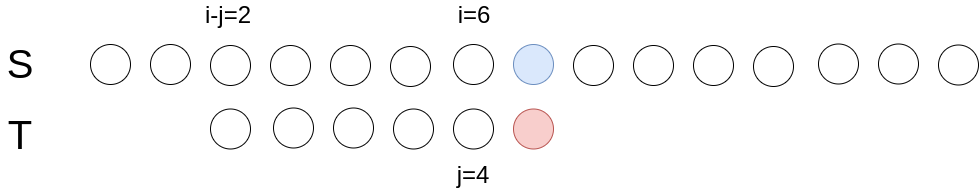
\includegraphics[scale=0.35]{pic1.png}
这个时候, 算法不是从$S[i-j+1]=S[3]$的位置和$T[0]$重新开始比较,而是设法让$T$向右滑动一段距离, 也就是让$S[i+1]$和$T[k+1]$来比较. 像下面这个样子: \par
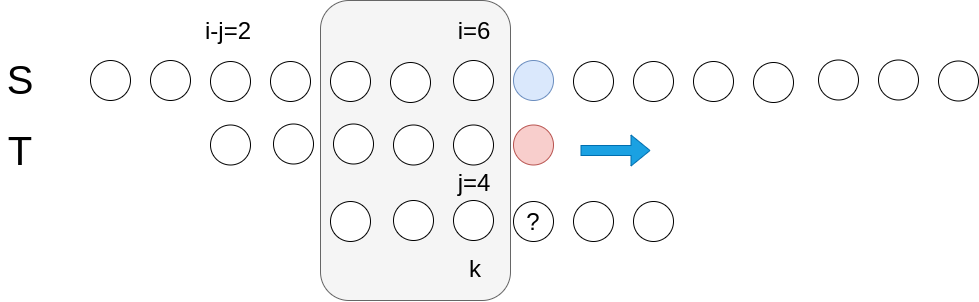
\includegraphics[scale=0.35]{pic2.png} \par
为了能够直接判断$S[i+1]$是否等于$T[k+1]$,需要满足上面方框中的部分相等. 那么只需要满足$SubT(j-k,j)=SubT(0,k)$. 可以发现, 这是在串$T$ 上的一个关系,跟$S$没有关系. 假设现在有了这个关系, 记作数组$f$,其中$k+1=f[j+1]$.  \par

比如对于串"abaabcac", 它的$f$ 数组是下面这样: \par

$\begin{matrix} 
index & 0 & 1 & 2 & 3 & 4 & 5 & 6 & 7 \\ 
string & a & b & a & a & b & c & a & c \\ 
f & -1 & 0 & 0 & 1 & 1 & 2 & 0 & 1 \\
\end{matrix}$

 有了这个$f$数组,寻找T在S中第一次出现的算法如下:\par
\begin{lstlisting}[language=C++, caption={FindFirstPos in S}]

int FindFirstPos(const std::string &S, const std::string &T,
                 const std::vector<int> &f) {
  const int lens = static_cast<int>(S.size());
  const int lent = static_cast<int>(T.size());
  int i = 0, j = 0;
  while (i < lens) {
    if (j == -1 || S[i] == T[j]) {
      i++;
      j++;
    } else {
      j = f[j];
    }
    if (j >= lent) {
      return i - lent;
    }
  }
  return -1;
}
\end{lstlisting}

\section{$f$数组计算}
首先$f[0]=-1$. 假设现在已经计算了$f[1],f[2],..,f[j]$,令$k=f[j]$. 现在来看$f[j+1]$. 由于$k=f[j]$,那么有下面的条件满足: \par
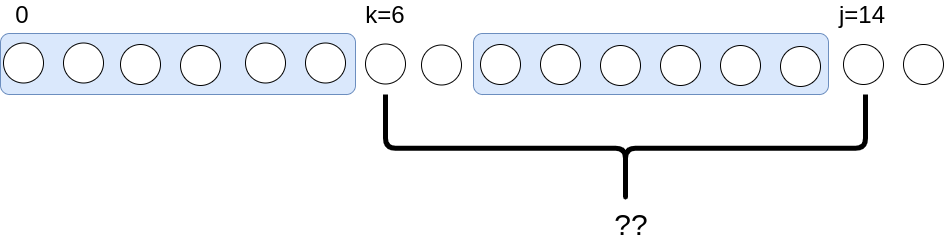
\includegraphics[scale=0.35]{pic3.png} \par
$Sub(0,k-1)=Sub(j-k,j-1)$,即两个蓝色框里面的串是相等的. 下面来检查$T[k]$和$T[j]$是否相等: \par
第一种情况,$T[j]==T[k]$,此时$f[j+1]=k+1$. 即下面两个粉色框里面的串相等. \par
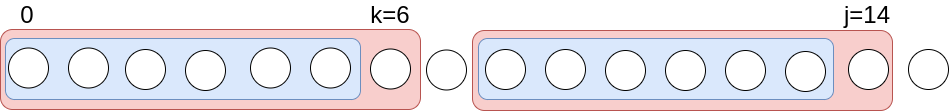
\includegraphics[scale=0.35]{pic4.png} \par
第二种情况,$T[j] \neq T[k]$,那么如下图所示, 需要找到一个位置$p$满足满足两个条件: \par

i $Sub(0,p)=Sub(j-(p+1),j-1)$, 即两个黄色方框相等 \par

ii $T[p+1]=T[j]$ \par
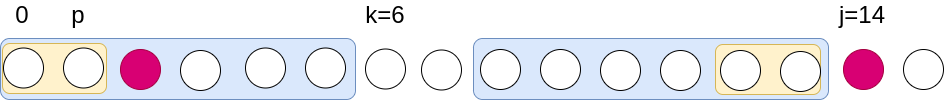
\includegraphics[scale=0.35]{pic5.png} \par
如果要使得第一个条件满足,那么如下图所示这三个黄色方框里面的串应该相等, 所以$p$应该满足$p+1=f[k]$. \par
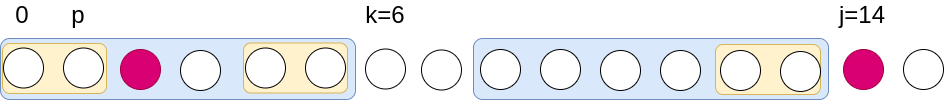
\includegraphics[scale=0.35]{pic6.png} \par
按照这样依次迭代下去, 直到找到一个位置满足条件2, 那么就找到了$f[j+1]$. \par
下面是计算$f$的代码: \par
\begin{lstlisting}[language=C++, caption={Compute $f$}]
std::vector<int> GetF(const std::string &T) {
  const int lent = static_cast<int>(T.size());
  std::vector<int> f(lent);
  f[0] = -1;
  int i = 0, j = -1;
  while (i + 1 < lent) {
    if (j == -1 || T[i] == T[j]) {
      f[++i] = ++j;
    } else {
      j = f[j];
    }
  }
  return f;
}
\end{lstlisting}

\section{进一步思考}
上面求出的$f$数组有一些缺陷。我们设T="aaaab",那么我们求出的$f$如下: \par

$\begin{matrix}
index & 0 & 1 & 2 & 3 & 4 \\ 
string & a & a & a & a & b \\ 
f & -1 & 0 & 1 & 2 & 3 
\end{matrix}$

那么在匹配的时候,假设匹配到$T[3]$的时候失配了,那么按照$f$数组,接下来,我们将比较$T[2]$和S的那个字母,很明显又失败了(因为$T[2],T[3]$都是a),接着比较$T[1],T[0]$,依次都失败了。这就是出现的问题。针对这个问题,对$F$数组进行以下改进: \par
\begin{lstlisting}[language=C++, caption={Batter algorithm to compute $f$}]
std::vector<int> FastF(const std::string &T) {
  const int lent = static_cast<int>(T.size());
  std::vector<int> f(lent);
  f[0] = -1;
  int i = 0, j = -1;
  while (i + 1 < lent) {
    if (j == -1 || T[i] == T[j]) {
      i++;
      j++;
      if (T[i] != T[j]) {
        f[i] = j;
      } else {
        f[i] = f[j];
      }
    } else {
      j = f[j];
    }
  }
  return f;
}
\end{lstlisting}
现在对于T="aaaab"求出的$f$数组为: \par

$\begin{matrix}
index & 0 & 1 & 2 & 3 & 4 \\ 
string & a & a & a & a & b \\ 
f & -1 & -1 & -1 & -1 & 3 
\end{matrix}$

\end{document}
